\documentclass[tikz,border=10pt]{standalone}
\usepackage{tikz}
\usepackage{slashed}
\usepackage{tikz-feynman}
\usetikzlibrary{positioning}
\usetikzlibrary{graphs}

\begin{document}

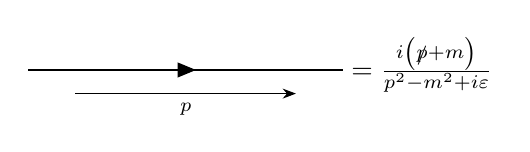
\begin{tikzpicture}[baseline]
	\begin{feynman}
		%% fig a
		\vertex (a1) at (0,0);
		\vertex[right =4cm  of a1] (a5);
		% 对各个顶点连线
		\diagram*{
		{ [edge= fermion]
		(a1) --[ momentum'={\scriptsize \(p\)}]  (a5),
		},
		};
	\end{feynman}
    \node at (5,2pt) {$=\frac{i \left( \slashed{p}+m \right)}{p^2-m^2+i\varepsilon }$};
\end{tikzpicture}

\end{document}
